\chapter{Related work}

\section{Image forgery}

When dealing with a digital image, it is quite common to wonder if it is original or has been counterfeited in some way. Images and videos have become the main information carriers in the digital era and used to store real world events, but  they are very easy to manipulate because of the availability of the powerful editing software and sophisticated digital cameras.

The contexts where doctored pictures could be involved are very disparate; they could be used in a tabloid or in an advertising poster or included in a journalistic report but also in a court of law where digital (sometimes printed) images are presented as crucial evidences for a trial in order to influence the final judgement. So, especially in the last case, reliably assessing image integrity becomes of fundamental importance. 

\emph{Image forensics} specifically deals with such issues by studying and developing technological tools which generally permit determining, by only analyzing a digital photograph (i.e., its pixels), if that asset has been manipulated or even which could have been the adopted acquisition device (such an issue is not relevant to the topic of the present paper). Moreover, if it has been established that something has been altered, it could be important to understand in which part of the image itself such a modification occurred, for instance, if a person or a specific object has been covered, if an area of the image has been cloned, if something (i.e., a face or a weapon) has been copied from another different image, or, even more, if a mixture of these processes has been carried out. 

\section{Image forgery detection techniques}

To verify the authenticity of a picture many techniques have been identified that can be categorized into active (intrusive) and blind (non-intrusive).

Operative techniques involve a phase of preprocessing the image itself at the time of its creation in order to include some additional information that will be used during the analysis phase. An example of operative technique is the watermarking.

Passive techniques analyze the content of the image using various statistics or semantic content in order to identify inconsistencies of some kind. This approach does not alter the contents of the image.
There is a general technique, suitable to capture all kinds of inconsistencies present in an image, but each different method specialises in the identification of a particular type.

\section{Image splicing}

Image splicing is a very common type of infringement which basically consists in copying a region of a given image to another, thus creating a composition of two different pictures together.

\begin{figure}
  \centering
    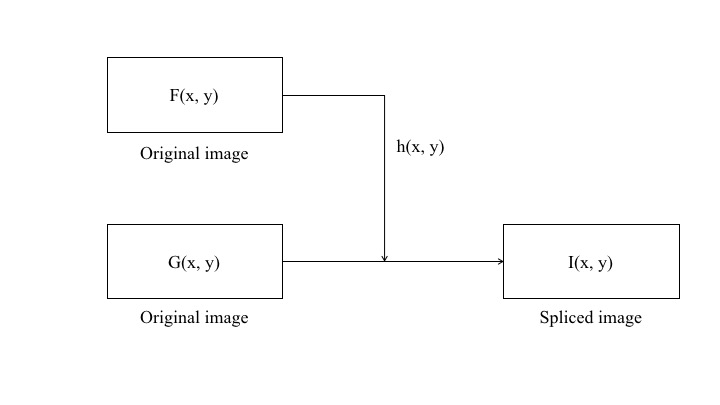
\includegraphics[width=0.8\textwidth]{imagesplicing}
    \caption{Image splicing process}
\end{figure}

Image splicing consists of using parts of two or more images to compose a new image that never took place in space and time. 

This composition process includes all the necessary operations (such as brightness and contrast adjustment, affine transformations, color changes, etc.) to construct realist images able to deceive viewer. In this process, normally, we refer to the parts coming from other images as aliens and the image receiving the other parts as host.

One of the common studied case is image composition involving people are very popular and are employed with very different objectives. 

\subsubsection{Some famous cases}

Photography has lost its innocence since the early days of his birth. In fact already in 1860, only a few decades after Niépce created the first photo, the first manipulated photographs were identified in 1826. With the advent of digital cameras, camcorders and sophisticated photo editing software, digital image manipulation is becoming more common. 

\paragraph{O.J. Simpson - June 1994}

This altered photography O.J. Simpson appeared on the cover of the magazine Time Magazine, soon after his arrest for murder. 

\begin{wrapfigure}{r}{0.5\textwidth}
  \begin{center}
    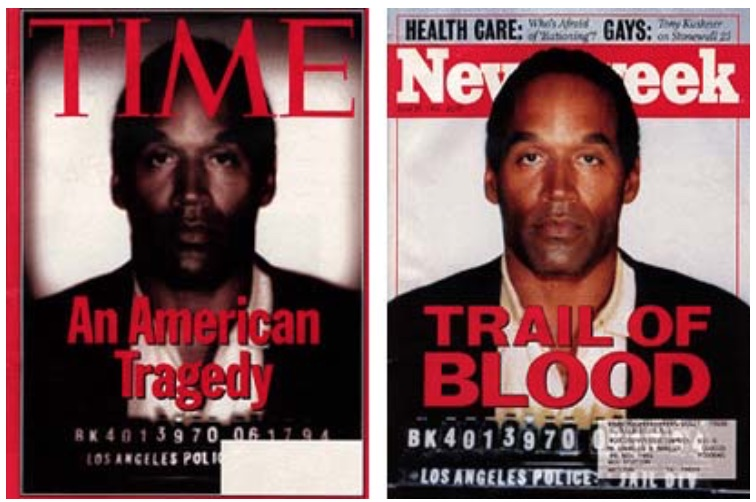
\includegraphics[width=0.48\textwidth]{ojsimpson}
  \end{center}
  \caption{The Time Magazine and O.J. Simpson}
  \vspace{-1cm}
\end{wrapfigure}

In fact, the photograph was altered compared to the original image that has appeared on the cover of Newsweek magazine. Time magazine was accused of manipulation of the photography in order to make darker and menacing figure of Simpson.

\paragraph{Iraq - April 2003}

This composition of a British soldier in Basra, which keeps pointing toward a civilian Iraqi gesticulates covered, she appeared on the cover of the Los Angeles Times, immediately after the invasion of Iraq. 

\begin{wrapfigure}{l}{0.5\textwidth}
  \begin{center}
    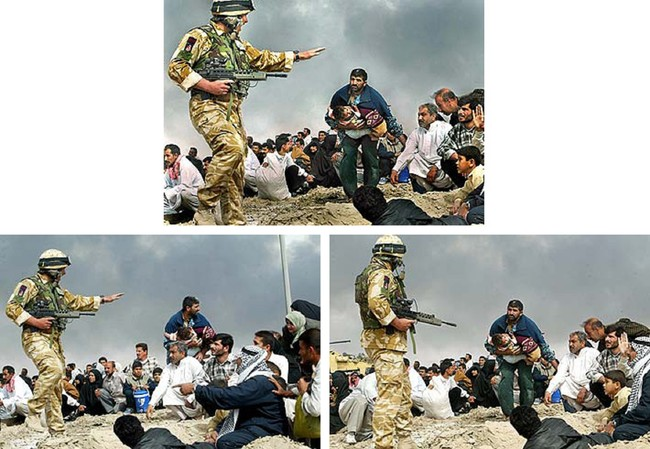
\includegraphics[width=0.48\textwidth]{iraq}
  \end{center}
  \caption{An example of image composition}
\end{wrapfigure}

Brian Walski, a staff photographer for the Los Angeles Times and a veteran of the news with thirty years of experience, was summarily fired from his publisher for their merged two of his shots in order to improve the composition.

\paragraph{George W. Bush - March 2004}

This image, taken from promo released for the election campaign of George w. Bush, outlined a packed audience of soldiers as a backdrop to a child who was flying the American flag. This image was digitally souped-up, using a crude copy and paste, removing Bush from the podium. 

\begin{wrapfigure}{r}{0.5\textwidth}
  \begin{center}
    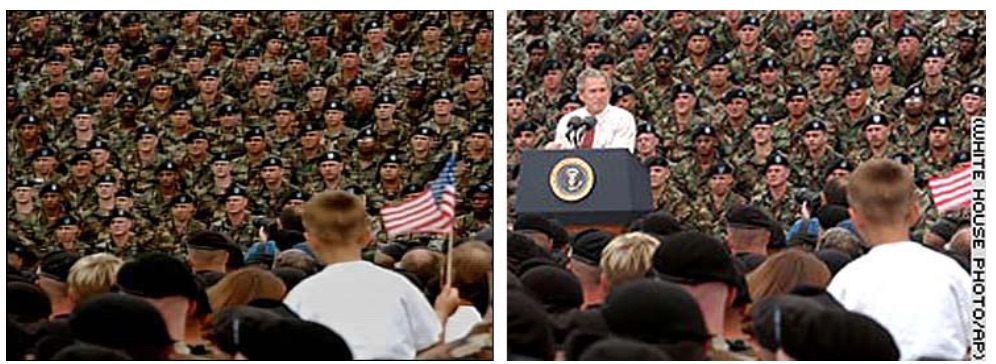
\includegraphics[width=0.48\textwidth]{bush}
  \end{center}
  \caption{An example of image composition}
\end{wrapfigure}


After admitting the tampering with the staff of the television station edited and sent to Bush promo with the original photo.

Cases such as this show how present image composition is in our daily lives. Unfortunately, it also decreases our trust on images and highlights the need for developing methods for recovering back such confidence.

\section{Methods based on light inconsistencies}

Methods for detecting image composition have become actual and powerful tools in the forensic analysis process. Different types of methods have been proposed for detecting image composition. Methods based on inconsistencies in compatibility metrics, JPEG compression features and perspective constraints are just a few examples of inconsistencies explored to detect forgeries.

After studying and analyzing the advantages and drawbacks of different types of methods for detecting image composition, this work herein relies on the research hypothesis that image illumination inconsistencies are strong and powerful evidence of image composition.

This hypothesis has already been used by some researchers in the literature whose work will be detailed in the next chapter, and it is specially useful for detecting image composition because, even for expert counterfeiters, a perfect illumination match is extremely hard to achieve. Also, there are some experiments that show how difficult is for humans perceive image illumination inconsistencies.

We can divide methods that explore illumination inconsistencies into three main groups of methods:
\begin{enumerate}
\item methods based on inconsistencies in the \textbf{light setting}: this group of methods encloses approaches that look for inconsistencies in the light position and in models that aim at reconstructing the scene illumination conditions.
\item methods based on inconsistencies in the \textbf{shadows}: this group of methods encloses approaches that look for inconsistencies in the scene illumination using telltales derived from shadows.
\item methods based on inconsistencies in \textbf{light color}: this group of methods encloses approaches that look for inconsistencies in the color of illuminants present in the scene.
\end{enumerate}


\subsection{Inconsistencies in the light setting}

Johnson and Farid\cite{Johnson:2005:EDF:1073170.1073171} proposed an approach based on illumination inconsistencies, looking for chromaticity aberrations as an indicator of image forgery. They analyzed the light source direction from different objects in the same image trying to detect traces of tampering. The authors start by imposing different constraints for the problem:

\begin{enumerate}
\item All the analyzed objects have \emph{Lambertian surface}\footnote{A Lambertian surface for reflection is a surface that appears uniformly bright from all directions of view and reflects the entire incident light. Lambertian reflectance is the property exhibited by an ideal matte or diffusely reflecting surface.}.
\item The surface reflectance is constant.
\item The object surface is illuminated by an infinitely distant light source.
\end{enumerate}

Using RGB images, the authors assume that the chromaticity deviation is constant (and dependent on each channel wavelength) for all color channels and create a model, based on image statistical properties, of how the ray light should split for each color channel. Given this premise and using the green channel as reference, the authors estimate deviations between the red and green channels and between the blue and green channels for selected parts of the image. Inconsistencies on this split pattern are used as telltales to detect forgeries. 

A drawback of this method is that chromaticity deviation depends on the camera lens used to take the picture. 

\subsection{Inconsistencies in the shadows}

Another set of methods is based on inconsistencies on the shadows in the image.
 
Zhang and Wang \cite{zhang2009detecting} proposed an approach that utilizes the planar homology\cite{springer1964geometry}, which models the relationship of shadows in an image for discovering forgeries.

Based on this model, the authors proposed to construct two geometric constraints: the first one is based on the relationship of connecting lines. A connecting line is a line that connects some object point with its shadow. According to planar homology, all of these connecting lines intersect in a vanishing point. 

\begin{figure}
  \centering
    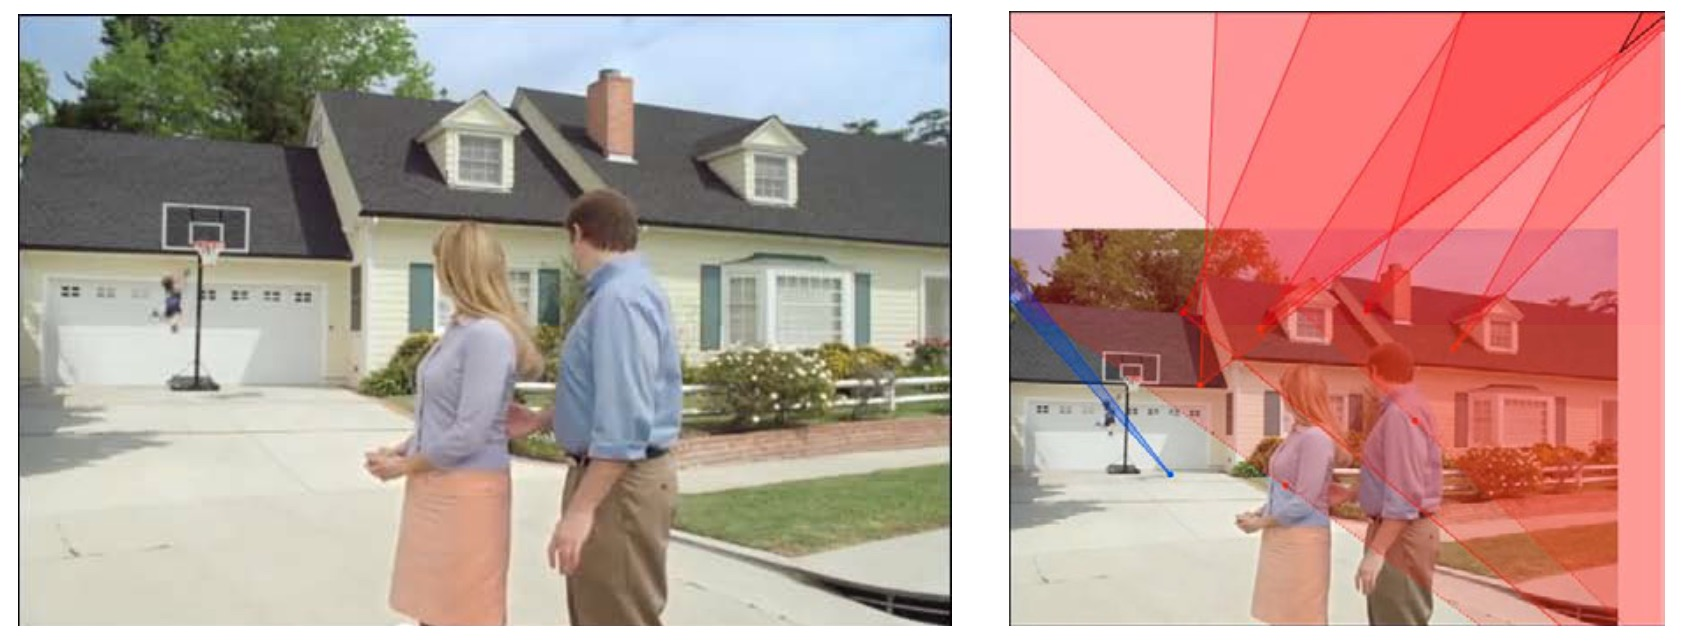
\includegraphics[width=0.8\textwidth]{shadows_inconsistencies}
    \caption{Original image (left) and the extracted shadows constraints (right)}
    \label{shadows_inconsistencies}
\end{figure}

The second constraint is based on the ratio of these connecting lines. In addition, the authors also proposed to explore the changing ratio along the normal direction of the shadow boundaries. 

Geometric and shadow photometric constraints together are used to detect image compositions. However, in spite of being a good initial step in forensic shadow analysis, the major drawback of the method is that it only works with images containing casting shadows, a very restricted scenario.

\subsection{Inconsistencies in light color}

The last group of methods investigate the presence, or not, of composition operations in digital images using color inconsistencies.

Gholap and Bora\cite{gholap2008illuminant} pioneered this approach using the \emph{illuminant colors}. For that, the authors used a \emph{dichromatic reflection model} proposed by Tominaga and Wandell\cite{tominaga1989standard}, which assumes a single light source to estimate illuminant colors from images.

\begin{wrapfigure}{l}{0.5\textwidth}
  \begin{center}
    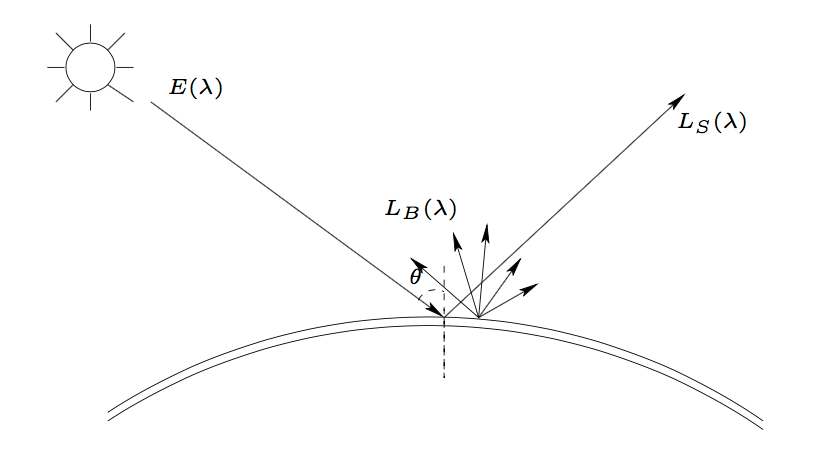
\includegraphics[width=0.48\textwidth]{dichromatic_reflection_model}
  \end{center}
  \label{dichromatic_reflection_model}
  \caption{The dichromatic reflection model}
\end{wrapfigure}


According to this model, reflection of any non-homogeneous materials may be modelled as additive mixture of two components, diffused reflection and surface reflection as shown in Fig. \ref{dichromatic_reflection_model}.

Considering an object point illuminated by a light source, the reflected ray consists of diffuse reflection $L_B (\lambda)$ and surface reflection $L_S (\lambda)$. The reflected light $L(\Theta, \lambda)$ can be written as:

\begin{equation}
L(\Theta, \lambda) = m_S(\Theta) L_S(\lambda) + m_B(\Theta) L_B(\lambda)
\end{equation}

where $m_S(\Theta)$ and $m_B(\Theta)$ are geometrical factors and $\Theta$ the angle of the incident light. This equation can be rewritten in terms of RGB sensors in matrix form.

The two vectors $L_B(\lambda)$ and $L_S(\lambda)$ span the two dimensional plane called \emph{dichromatic plane}.

Dichromatic planes can also be estimated using principal component analysis (PCA) from each specular highlight region of an image. By applying a \emph{Singular Value Decomposition (SVD)} on the RGB matrix extracted from highlighted regions, the authors extract the eigenvectors associated with the two most significant eigenvalues to construct the \emph{dichromatic plane}. This plane is then mapped onto a straight line, named dichromatic line, in normalized \emph{r-g-chromaticity} space. 

For distinct objects illuminated by the same light source, the intersection point produced by their dichromatic line intersection represents the illuminant color. If the image has more than one illuminant, it will present more than one intersection point, which is not expected to happen in pristine (non-forged images). This method represented the first important step toward forgery detection using illuminant colors, but has some limitations such as the need of well defined specular highlight regions for estimating the illuminants.





\subsection{Illuminant Maps}

\subsubsection{Generalized Greyworld algorithm}

\subsubsection{Inverse Intensitiy Chromaticiy}


\subsection{Human faces splicing detection}

\subsection{Region splicing detection}